% Created 2016-08-17 Wed 14:38
\documentclass[tikz]{standalone}

\usepackage[utf8]{inputenc}
\usepackage[T1]{fontenc}

\usepackage{circledsteps}

\RequirePackage{xcolor}

%% HPI color definitions according to the design manual
% These do not exactly match the RGB values used in the Powerpoint slide master due to unknown reasons
\definecolor{hpiyellow}{RGB}{246,168,0}
\definecolor{hpiorange}{RGB}{221,97,8}
\definecolor{hpired}{RGB}{177,6,58}
\definecolor{hpigray}{RGB}{90,96,101}
\definecolor{hpiblue}{RGB}{0,122,158}


\renewcommand{\sfdefault}{neosans}
% Different font weights for neosans
\newcommand{\textl}[1]{{\fontseries{l}\selectfont #1}} % light
\newcommand{\textm}[1]{{\fontseries{m}\selectfont #1}} % medium, same as default weight
\newcommand{\textsb}[1]{{\fontseries{sb}\selectfont #1}} % semibold
\newcommand{\textmb}[1]{{\fontseries{mb}\selectfont #1}} % bold, same as \textbf
\newcommand{\texteb}[1]{{\fontseries{eb}\selectfont #1}} % extra bold
\newcommand{\textub}[1]{{\fontseries{ub}\selectfont #1}} % ultra bold

\tikzset{every picture/.style={/utils/exec={\sffamily}}}
\tikzset{flipflop RSflanke/.style={
  flipflop,
  flipflop def={t1=S, t2=C, c2=1, t3=R, t6=Q, t4={\ctikztextnot{Q}}}
}}


\tikzset{
  mechanicalSwitch/.pic={
    \coordinate (-inUp) at (135:2); 
    \coordinate (-inDown) at (235:2);
    \coordinate (-out) at (2,0);
    \coordinate (-center) at (0,0);
    
    \draw (0,0) circle [radius = 2cm];
    \draw [fill=gray!20] (0,0) circle [radius = 0.2cm];

    \draw (0, 0) -- (2, 0);
    \draw (135:.8) -- (135:2); 
    \draw (225:.8) -- (225:2); 

    \draw [fill=gray!20] (2, 0) circle [radius=0.05cm]; 
    \draw [fill=gray!20] (135:2) circle [radius=0.05cm]; 
    \draw [fill=gray!20] (225:2) circle [radius=0.05cm]; 

    
    \draw [thick] (0,0) -- (175:1.5); 

    \draw [dashed, <->, domain=135:225] plot ({cos(\x)}, {sin(\x)}); 
  },
  mechanicalSwitchClosed/.pic={
    \coordinate (-inUp) at (135:2); 
    \coordinate (-inDown) at (255:2);
    \coordinate (-out) at (2,0);
    \coordinate (-center) at (0,0);
    \draw (0,0) circle [radius = 2cm];
    \draw [fill=gray!20] (0,0) circle [radius = 0.2cm];

    \draw (0, 0) -- (2, 0);
    \draw (135:.8) -- (135:2); 
    \draw (225:.8) -- (225:2); 

    \draw [fill=gray!20] (2, 0) circle [radius=0.05cm]; 
    \draw [fill=gray!20] (135:2) circle [radius=0.05cm]; 
    \draw [fill=gray!20] (225:2) circle [radius=0.05cm]; 

    
    \draw [thick] (0,0) -- (135:2); 

    \draw [dashed, <->, domain=135:225] plot ({cos(\x)}, {sin(\x)}); 
  }
}


\usetikzlibrary{calc}
\usetikzlibrary{positioning}

\usepackage{ifthen}
\usetikzlibrary{decorations.pathreplacing,decorations.pathmorphing,calc}

\newcommand{\pplusa}[6]{%
  % #1: offset, #2: fill color #3: packet length #4: ACK length, #5 label
  % #6: X to loose the ACK 
  
  \coordinate (pStartSend_#5) at ($(a) + (0,-0.5)-(0,#1)$); 
  \coordinate (pEndSend_#5) at  ($  (pStartSend_#5) + (0,-#3) $ ); 
  \coordinate (pStartReceive_#5) at ($ (pStartSend_#5) + (3.5,-1) $); 
  \coordinate (pEndReceive_#5) at ($  (pStartReceive_#5) + (0,-#3) $ ); 
  \coordinate (aStartSend_#5) at ($(b) +  (0,-0.5)-(0,#1)-(0,1)-(0,#3)  $); 
  \coordinate (aEndSend_#5) at ($ (aStartSend_#5)  + (0,-#4) $); 
  \coordinate (aStartReceive_#5) at ($ (aStartSend_#5) + (-3.5,-1)  $); 
  \coordinate (aEndReceive_#5) at ($ (aStartReceive_#5) + (0,-#4)  $);   

  
  % Packets: 
  \ifthenelse{\equal{#6}{X}}
  {
    % packet gets lost
    \coordinate (pStartLoss_#5) at ($ (pStartSend_#5) + (1.75,-1)  $); 
    \coordinate (pEndLoss_#5) at ($ (pStartLoss_#5) + (0,-#3)  $);

    \draw [fill=#2, semitransparent] (pStartSend_#5) --
    (pStartLoss_#5) decorate [decoration=zigzag] {-- (pEndLoss_#5)}
    -- (pEndSend_#5);
  \node at ($(1.75,-0.5) - (0,#1) - (0,0.5*#3) -(0, 0.5)$) {P\,#5 lost!}; 
    
  }
  {
    % packet normally delivered
  \draw [fill=#2, semitransparent] (pStartSend_#5) -- (pStartReceive_#5) -- (pEndReceive_#5) -- (pEndSend_#5);
  \node at ($(1.75,-0.5) - (0,#1) - (0,0.5*#3) -(0, 0.5)$) {P\,#5}; 
  \draw [->] (a) ++ (pStartSend_#5) -- (pStartReceive_#5); 
  \draw [->] (a) ++ (pEndSend_#5) -- (pEndReceive_#5); 

  % ACK:
    %ACK normally sent: 
  \draw [fill=#2, semitransparent] (aStartSend_#5) -- (aStartReceive_#5) -- (aEndReceive_#5) -- (aEndSend_#5); 


  \draw [->] (aStartSend_#5) -- (aStartReceive_#5); 
  \draw [->] (aEndSend_#5) -- (aEndReceive_#5); 
}

}

\begin{document}

% \begin{tikzpicture}

%   \node [fill=hpiorange!10](a) {A};
%   \node [fill=hpiblue!10, right=3cm of a] (b) {B};

%   \draw (a) -- ++(0,-8); 
%   \draw (b) -- ++(0,-8);
  
%   \pplusa{0}{white}{0}{0}{1}{}
% \end{tikzpicture}


% \begin{tikzpicture}
%   \label{page:cc:one_cwnd_increase}
%   \node [fill=hpiorange!10](a) {A};
%   \node [fill=hpiblue!10, right=3cm of a] (b) {B};

%   \draw (a) -- ++(0,-18); 
%   \draw (b) -- ++(0,-18);
  
%   \pplusa{0}{white}{0}{0}{1}{}
%   % ----- 
%   \pplusa{4}{white}{0}{0}{2}{}
%   \pplusa{4.1}{white}{0}{0}{3}{}
%   % ----- 
%   \pplusa{8}{white}{0}{0}{4}{}
%   \pplusa{8.1}{white}{0}{0}{5}{}
%   \pplusa{8.2}{white}{0}{0}{6}{}
%   % ----- 
%   \pplusa{12}{white}{0}{0}{7}{}
%   \pplusa{12.1}{white}{0}{0}{8}{}
%   \pplusa{12.2}{white}{0}{0}{9}{}
%   \pplusa{12.3}{white}{0}{0}{10}{}

% \end{tikzpicture}



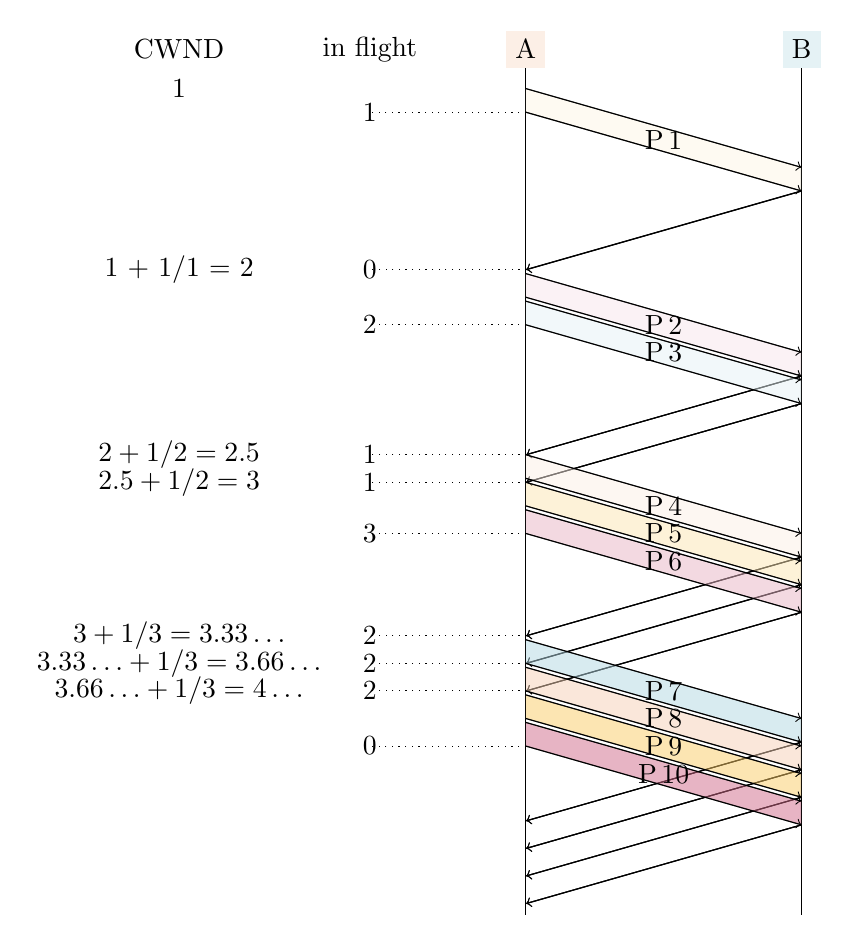
\begin{tikzpicture}
  \label{page:cc:one_cwnd_increase:exact:comments}
  \node [fill=hpiorange!10](a) {A};
  \node [fill=hpiblue!10, right=3cm of a] (b) {B};

  \node [left=of a] (inflight) {in flight}; 
  \node [left=of inflight] (cwnd) {CWND}; 
  \draw (a) -- ++(0,-11); 
  \draw (b) -- ++(0,-11);
  
  \pplusa{0}{hpiyellow!10}{0.3}{0}{1}{}
  \node at (cwnd |- pStartSend_1)  {1};
  \draw [dotted] (pEndSend_1) -- (inflight |- pEndSend_1) node  {1};
  
  % ----- after one RTT: 

  \node at (cwnd |- aEndReceive_1)  {1 + 1/1 = 2};
  \draw [dotted] (aEndReceive_1) -- (inflight |- aEndReceive_1) node  {0};
  
  \pplusa{2 + 0.3 + 0.05}{hpired!10}{0.3}{0}{2}{}
  
  \pplusa{2 + 2*0.3 + 2*0.05}{hpiblue!10}{0.3}{0}{3}{}
  \draw [dotted] (pEndSend_3) -- (inflight |- pEndSend_3) node  {2};


  
  % ----- after two RTTs: 
  \node at (cwnd |- aEndReceive_2)  {$2 + 1/2 = 2.5$};
  \draw [dotted] (aEndReceive_2) --  (inflight |- aEndReceive_2) node {1};


  
  \pplusa{2*2 + 2*0.3 + 1*0.05}{hpiorange!10}{0.3}{0}{4}{}

  \node at (cwnd |- aEndReceive_3)  {$2.5 + 1/2 = 3 $};
  \draw [dotted] (aEndReceive_3) --  (inflight |- aEndReceive_3) node {1};



  \pplusa{2*2 + 3*0.3 + 2*0.05}{hpiyellow!30}{0.3}{0}{5}{}
  \pplusa{2*2 + 4*0.3 + 3*0.05}{hpired!30}{0.3}{0}{6}{}

  \draw [dotted] (pEndSend_6) -- (inflight |- pEndSend_6) node  {3};
  
  % % ----- nach 3 RTTs
  \node at (cwnd |- aEndReceive_4)  {$3 + 1/3 = 3.33\dots  $};
  \draw [dotted] (aEndReceive_4) --  (inflight |- aEndReceive_4) node {2};
  
  
  \pplusa{3*2 + 3*0.3 + 2*0.05}{hpiblue!30}{0.3}{0}{7}{}

  \node at (cwnd |- aEndReceive_5)  {$3.33\dots  + 1/3 = 3.66\ldots $};
  \draw [dotted] (aEndReceive_5) --  (inflight |- aEndReceive_5) node {2};
  
  \pplusa{3*2 + 4*0.3 + 3*0.05}{hpiorange!30}{0.3}{0}{8}{}

  \node at (cwnd |- aEndReceive_6)  {$3.66\dots  + 1/3  = 4\ldots $};
  \draw [dotted] (aEndReceive_6) --  (inflight |- aEndReceive_6) node {2};

  \pplusa{3*2 + 5*0.3 + 4*0.05}{hpiyellow!60}{0.3}{0}{9}{}

  \pplusa{3*2 + 6*0.3 + 5*0.05}{hpired!60}{0.3}{0}{10}{}
  \draw [dotted] (pEndSend_10) -- (inflight |- pEndSend_10) node  {0};


\end{tikzpicture}


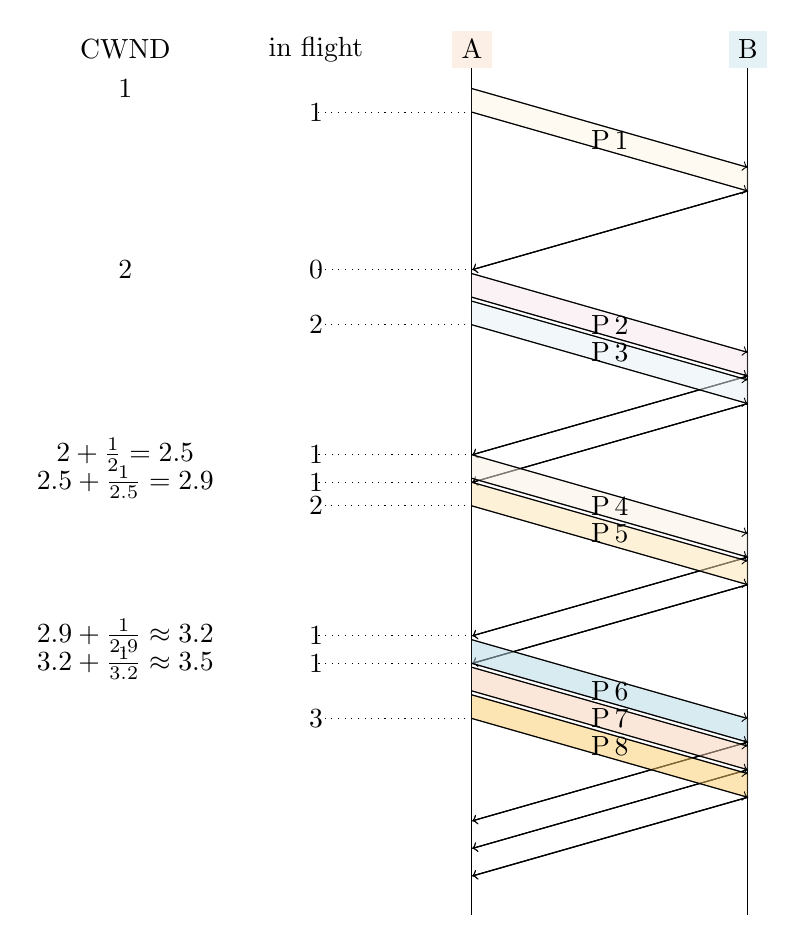
\begin{tikzpicture}
  \label{page:cc:one_cwnd_increase:exact:comments}
  \node [fill=hpiorange!10](a) {A};
  \node [fill=hpiblue!10, right=3cm of a] (b) {B};

  \node [left=of a] (inflight) {in flight}; 
  \node [left=of inflight] (cwnd) {CWND}; 
  \draw (a) -- ++(0,-11); 
  \draw (b) -- ++(0,-11);
  
  \pplusa{0}{hpiyellow!10}{0.3}{0}{1}{}
  \node at (cwnd |- pStartSend_1)  {1};
  \draw [dotted] (pEndSend_1) -- (inflight |- pEndSend_1) node  {1};
  
  % ----- after one RTT: 

  \node at (cwnd |- aEndReceive_1)  {2};
  \draw [dotted] (aEndReceive_1) -- (inflight |- aEndReceive_1) node  {0};
  
  \pplusa{2 + 0.3 + 0.05}{hpired!10}{0.3}{0}{2}{}
  
  \pplusa{2 + 2*0.3 + 2*0.05}{hpiblue!10}{0.3}{0}{3}{}
  \draw [dotted] (pEndSend_3) -- (inflight |- pEndSend_3) node  {2};


  
  % ----- after two RTTs: 
  \node at (cwnd |- aEndReceive_2)  {$2 + \frac{1}{2} = 2.5$};
  \draw [dotted] (aEndReceive_2) --  (inflight |- aEndReceive_2) node {1};


  
  \pplusa{2*2 + 2*0.3 + 1*0.05}{hpiorange!10}{0.3}{0}{4}{}

  \node at (cwnd |- aEndReceive_3)  {$2.5 + \frac{1}{2.5} = 2.9 $};
  \draw [dotted] (aEndReceive_3) --  (inflight |- aEndReceive_3) node {1};



  \pplusa{2*2 + 3*0.3 + 2*0.05}{hpiyellow!30}{0.3}{0}{5}{}
  % \pplusa{2*2 + 4*0.3 + 3*0.05}{hpired!30}{0.3}{0}{6}{}

  \draw [dotted] (pEndSend_5) -- (inflight |- pEndSend_5) node  {2};
  
  % % ----- nach 3 RTTs
  \node at (cwnd |- aEndReceive_4)  {$2.9 + \frac{1}{2.9} \approx 3.2 $};
  \draw [dotted] (aEndReceive_4) --  (inflight |- aEndReceive_4) node {1};
  
  
  \pplusa{3*2 + 3*0.3 + 2*0.05}{hpiblue!30}{0.3}{0}{6}{}

  \node at (cwnd |- aEndReceive_5)  {$3.2 + \frac{1}{3.2} \approx 3.5 $};
  \draw [dotted] (aEndReceive_5) --  (inflight |- aEndReceive_5) node {1};
  
  \pplusa{3*2 + 4*0.3 + 3*0.05}{hpiorange!30}{0.3}{0}{7}{}
  \pplusa{3*2 + 5*0.3 + 4*0.05}{hpiyellow!60}{0.3}{0}{8}{}

  \draw [dotted] (pEndSend_8) -- (inflight |- pEndSend_8) node  {3};

  % \pplusa{3*2 + 6*0.3 + 5*0.05}{hpired!60}{0.3}{0}{10}{}

\end{tikzpicture}


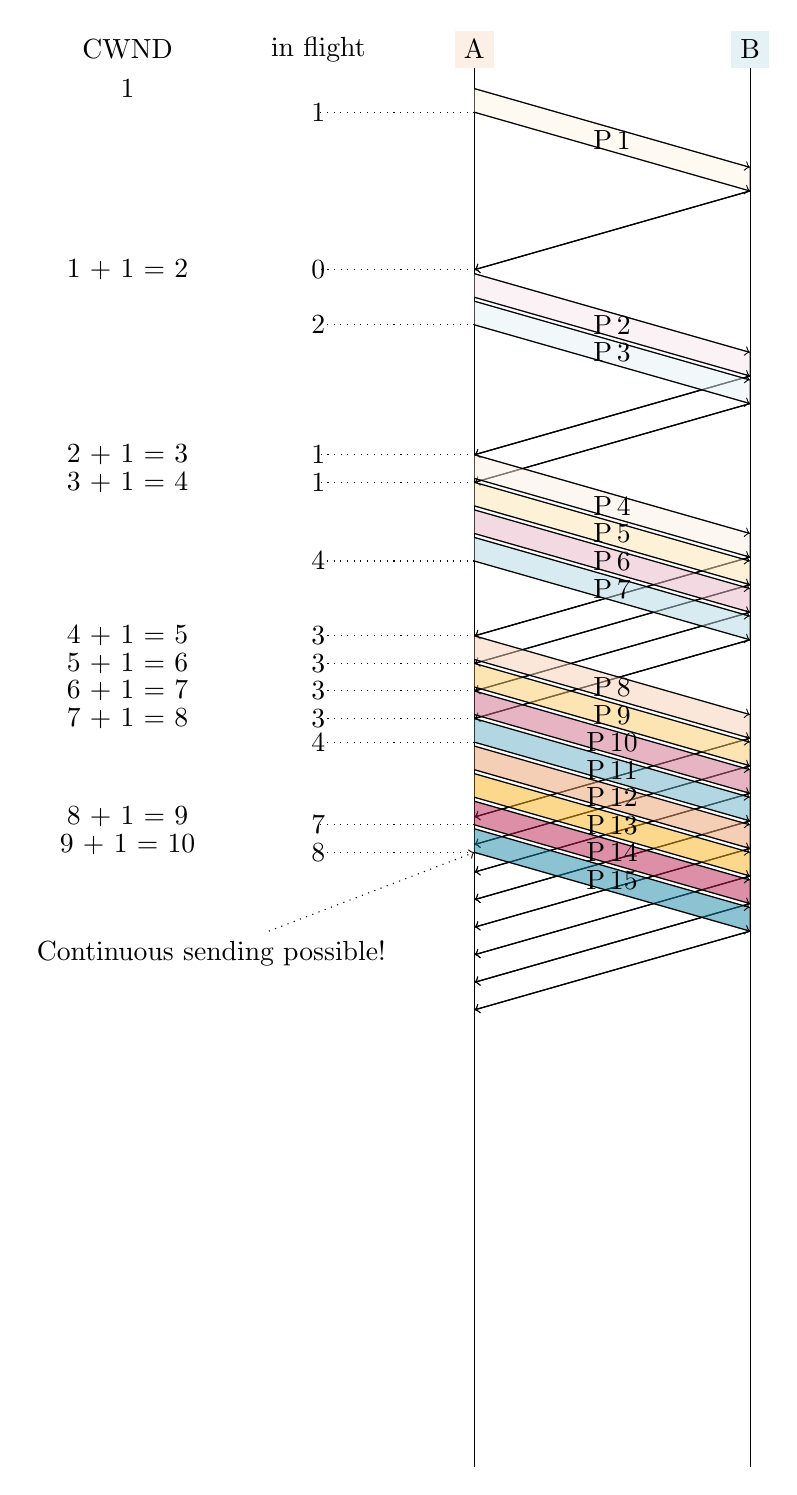
\begin{tikzpicture}
  \label{page:cc:slowstart:comments}
  \node [fill=hpiorange!10](a) {A};
  \node [fill=hpiblue!10, right=3cm of a] (b) {B};

  \node [left=of a] (inflight) {in flight}; 
  \node [left=of inflight] (cwnd) {CWND}; 
  \draw (a) -- ++(0,-18); 
  \draw (b) -- ++(0,-18);
  
  \pplusa{0}{hpiyellow!10}{0.3}{0}{1}{}
  \node at (cwnd |- pStartSend_1)  {1};
  \draw [dotted] (pEndSend_1) -- (inflight |- pEndSend_1) node  {1};
  
  % ----- after one RTT: 

  \node at (cwnd |- aEndReceive_1)  {1 + 1 = 2};
  \draw [dotted] (aEndReceive_1) -- (inflight |- aEndReceive_1) node  {0};
  
  \pplusa{2 + 0.3 + 0.05}{hpired!10}{0.3}{0}{2}{}
  
  \pplusa{2 + 2*0.3 + 2*0.05}{hpiblue!10}{0.3}{0}{3}{}
  \draw [dotted] (pEndSend_3) -- (inflight |- pEndSend_3) node  {2};


  
  % ----- after two RTTs: 
  \node at (cwnd |- aEndReceive_2)  {2 + 1 = 3};
  \draw [dotted] (aEndReceive_2) --  (inflight |- aEndReceive_2) node {1};


  
  \pplusa{2*2 + 2*0.3 + 1*0.05}{hpiorange!10}{0.3}{0}{4}{}

  \node at (cwnd |- aEndReceive_3)  {3 + 1 =  4};
  \draw [dotted] (aEndReceive_3) --  (inflight |- aEndReceive_3) node {1};



  \pplusa{2*2 + 3*0.3 + 2*0.05}{hpiyellow!30}{0.3}{0}{5}{}
  \pplusa{2*2 + 4*0.3 + 3*0.05}{hpired!30}{0.3}{0}{6}{}
  \pplusa{2*2 + 5*0.3 + 4*0.05}{hpiblue!30}{0.3}{0}{7}{}
  

  \draw [dotted] (pEndSend_7) -- (inflight |- pEndSend_7) node  {4};
  
  % % ----- nach 3 RTTs
  \node at (cwnd |- aEndReceive_4)  {4 + 1 = 5};
  \draw [dotted] (aEndReceive_4) --  (inflight |- aEndReceive_4) node {3};
  
  

  \node at (cwnd |- aEndReceive_5)  {5 + 1 = 6};
  \draw [dotted] (aEndReceive_5) --  (inflight |- aEndReceive_5) node {3};
  
  \pplusa{3*2 + 3*0.3 + 1*0.05}{hpiorange!30}{0.3}{0}{8}{}

  \node at (cwnd |- aEndReceive_6)  {6 + 1 = 7};
  \draw [dotted] (aEndReceive_6) --  (inflight |- aEndReceive_6) node {3};

  \pplusa{3*2 + 4*0.3 + 2*0.05}{hpiyellow!60}{0.3}{0}{9}{}

  \node at (cwnd |- aEndReceive_7)  {7 + 1 = 8};
  \draw [dotted] (aEndReceive_7) --  (inflight |- aEndReceive_7) node {3};

  
  \pplusa{3*2 + 5*0.3 + 3*0.05}{hpired!60}{0.3}{0}{10}{}
  \pplusa{3*2 + 6*0.3 + 4*0.05}{hpiblue!60}{0.3}{0}{11}{}
  \draw [dotted] (pEndSend_11) -- (inflight |- pEndSend_11) node  {4};

  % and second half of the 8 CWND
  \pplusa{3*2 + 7*0.3 + 5*0.05}{hpiorange!60}{0.3}{0}{12}{}
  \pplusa{3*2 + 8*0.3 + 6*0.05}{hpiyellow!90}{0.3}{0}{13}{}
  \pplusa{3*2 + 9*0.3 + 7*0.05}{hpired!90}{0.3}{0}{14}{}

  \node at (cwnd |- aEndReceive_8)  {8 + 1 = 9};
  \draw [dotted] (pEndSend_14) -- (inflight |- pEndSend_14) node  {7};
  
  \node at (cwnd |- aEndReceive_9)  {9 + 1 = 10};
  \pplusa{3*2 + 10*0.3 + 8*0.05}{hpiblue!90}{0.3}{0}{15}{}
  \draw [dotted] (pEndSend_15) -- (inflight |- pEndSend_15) node  {8};


  \node [below left=of pEndSend_15, align=right] (label) {Continuous sending possible!};
  \draw [dotted, ->] (label) -- (pEndSend_15); 

  
  

\end{tikzpicture}



% \begin{tikzpicture}
%   \label{page:cc:slowstart}
%   \node [fill=hpiorange!10](a) {A};
%   \node [fill=hpiblue!10, right=3cm of a] (b) {B};

%   \draw (a) -- ++(0,-18); 
%   \draw (b) -- ++(0,-18);
  
%   \pplusa{0}{white}{0.3}{0}{1}{}
%   % ----- 
%   \pplusa{4}{white}{0.3}{0}{2}{}
%   \pplusa{4.1}{white}{0.3}{0}{3}{}
%   % ----- 
%   \pplusa{8}{white}{0.3}{0}{4}{}
%   \pplusa{8.1}{white}{0.3}{0}{5}{}
%   \pplusa{8.2}{white}{0.3}{0}{6}{}
%   \pplusa{8.3}{white}{0.3}{0}{7}{}
%   % ----- 
%   \pplusa{12}{white}{0.3}{0}{8}{}
%   \pplusa{12.1}{white}{0.3}{0}{9}{}
%   \pplusa{12.2}{white}{0.3}{0}{10}{}
%   \pplusa{12.3}{white}{0.3}{0}{11}{}
%   \pplusa{12.4}{white}{0.3}{0}{12}{}
%   \pplusa{12.5}{white}{0.3}{0}{13}{}
%   \pplusa{12.6}{white}{0.3}{0}{14}{}
%   \pplusa{12.7}{white}{0.3}{0}{15}{}

% \end{tikzpicture}


\end{document}